\documentclass[man,12pt,floatsintext]{apa7}

\usepackage[american]{babel}
\usepackage{csquotes}
\usepackage{amsmath}
\usepackage{booktabs}
\usepackage{threeparttable}
\usepackage{graphicx}
\usepackage[style=apa,backend=biber]{biblatex}
\DeclareLanguageMapping{american}{american-apa}
\addbibresource{references.bib}

\hypersetup{hidelinks}

\title{College Proximity and the Return to Schooling: A Replication of Card (1993)}

\shorttitle{COLLEGE PROXIMITY AND RETURNS}

\authorsnames{Research Team}

\authorsaffiliations{Department of Economics, Peking University}

\leftheader{Research Team}

\abstract{Does additional schooling raise earnings, and by how much? We replicate
Card's (1993) analysis of the return to schooling using the 3,010 men in the
National Longitudinal Survey Young Men cohort. We estimate the association
between years of schooling and log hourly wages with ordinary least squares,
first without covariates and then with demographic, regional, urban, and
experience controls. We then instrument schooling with an indicator for having
grown up near a four-year college. Instrumental-variables estimates are
substantially larger than the ordinary least squares estimates, consistent with
attenuation bias in conventional estimates, but they are also much less precise.
The exercise reproduces Card's published estimates and illustrates both the
promise and the fragility of college proximity as an instrument.}

\keywords{returns to schooling, instrumental variables, college proximity, replication}

\begin{document}

\maketitle

\section{Introduction}

The effect of education on income is one of the central questions in labor
economics. A long literature documents a robust positive association between
years of schooling and earnings, but whether this association is causal remains
contested because schooling is chosen and is correlated with unobserved ability,
family background, and local labor market conditions.

\Textcite{card1993} proposed an influential identification strategy based on
geographic variation in college proximity. Men who grew up near a four-year
college are more likely to attend college, so proximity predicts schooling.
If proximity affects wages only through its effect on schooling, the
college-proximity indicator can serve as an instrument for years of schooling.
Card reported ordinary least squares (OLS) returns of roughly 7\% and
instrumental-variables (IV) returns of 10--14\%.

In this note we replicate the core of Card's analysis with a single script. We
ask what the effect of education on income is, and we compare OLS, OLS with
covariates, and two-stage least squares (2SLS) estimates from the same sample.
Our contribution is pedagogical: the entire pipeline, from data preparation
through estimation, figures, tables, and the results paragraph, is reproduced
by \texttt{script/01\_card1993\_replication.R}.

\section{Data and Method}

The data are the NLS Young Men cohort extract analyzed by
\textcite{card1993}, distributed as the \texttt{card} data set in the
\texttt{wooldridge} package for R \parencite{wooldridge2010}. The sample
contains 3,010 men with valid hourly wages and years of schooling. Hourly wages
are measured in 1976 cents and are analyzed in logs. The sample is restricted
to men with complete data on all model variables; no observations are lost
because the variables used here are complete for the 3,010 men.

We estimate three models. Model 1 is the baseline OLS regression
\begin{equation}
  \ln(W_i) = \beta_0 + \beta_1 E_i + \varepsilon_i,
\end{equation}
where $W_i$ is the hourly wage and $E_i$ is years of schooling. Model 2 adds
covariates:
\begin{equation}
  \ln(W_i) = \beta_0 + \beta_1 E_i + \mathbf{X}_i'\boldsymbol{\gamma}
  + \varepsilon_i,
\end{equation}
where $\mathbf{X}_i$ includes indicators for being Black, living in the South,
living in a standard metropolitan statistical area (SMSA) in 1976 and in 1966,
indicators for eight of the nine census regions in 1966 (the Northeast is the
reference category), years of potential experience, and its square.

Model 3 treats schooling as endogenous and instruments it with
\texttt{nearc4}, an indicator equal to one if the man grew up in a local labor
market with a four-year college in 1966. The first stage is
\begin{equation}
  E_i = \pi_0 + \pi_1 Z_i + \mathbf{X}_i'\boldsymbol{\delta} + \nu_i,
\end{equation}
and the second stage replaces $E_i$ with its fitted value from
Equation~3, using the same covariates as Model 2. Standard errors are the
classical homoskedastic OLS and 2SLS standard errors, matching Card's
reported precision.

\section{Results}

Residence near a four-year college produces a larger estimated return to schooling than ordinary least squares, consistent with attenuation in the OLS estimates. Among the 3,010 men in the NLS Young Men cohort, one additional year of schooling is associated with 5.3\% higher hourly wages in the baseline model (\textit{b} = 0.052, \textit{SE} = 0.003, \textit{p} < .001) and 7.8\% higher wages after controlling for race, region, urban residence, and experience (\textit{b} = 0.075, \textit{SE} = 0.003, \textit{p} < .001). Instrumenting schooling with an indicator for growing up near a four-year college (nearc4) raises the return to 14.1\% (\textit{b} = 0.132, \textit{SE} = 0.055, \textit{p} = .017, 95\% CI [0.024, 0.239]); the instrument is not weak (first-stage \textit{F}(1, 2994) = 13.26, \textit{p} < .001). If college proximity affects wages only through schooling, the gap between the OLS and 2SLS estimates implies that conventional estimates understate the return to schooling by about 6 percentage points; the wide 2SLS interval and the local-average interpretation of the IV estimand nonetheless caution against treating 14\% as a population-wide causal effect.


Table~\ref{tab:returns} reports the full set of coefficients, standard errors,
and 95\% confidence intervals for the three models. Figure~\ref{fig:scatter}
shows the raw education--wage relationship, and Figure~\ref{fig:effects}
compares the schooling coefficient across models.

\begin{table}[htbp]
\centering
\begin{threeparttable}
\caption{Returns to Schooling Estimated by OLS and 2SLS}
\label{tab:returns}
\footnotesize
\setlength{\tabcolsep}{4pt}

\begin{tabular}[t]{lcccccc}
\toprule
\multicolumn{1}{c}{\textbf{ }} & \multicolumn{2}{c}{\textbf{Model 1 (OLS)}} & \multicolumn{2}{c}{\textbf{Model 2 (OLS)}} & \multicolumn{2}{c}{\textbf{Model 3 (2SLS)}} \\
\cmidrule(l{3pt}r{3pt}){2-3} \cmidrule(l{3pt}r{3pt}){4-5} \cmidrule(l{3pt}r{3pt}){6-7}
\multicolumn{1}{c}{Variable} & b (SE) & 95\% CI & b (SE) & 95\% CI & b (SE) & 95\% CI\\
\midrule
Years of schooling & .052 (.003) & {}[.046, .058] & .075 (.003) & {}[.068, .082] & .132 (.055) & {}[.024, .239]\\
Black & --- &  & -.199 (.018) & {}[-.235, -.163] & -.147 (.054) & {}[-.252, -.041]\\
South & --- &  & -.148 (.026) & {}[-.199, -.097] & -.145 (.027) & {}[-.198, -.091]\\
SMSA & --- &  & .136 (.020) & {}[.097, .176] & .112 (.032) & {}[.050, .174]\\
SMSA in 1966 & --- &  & .026 (.019) & {}[-.012, .064] & .019 (.022) & {}[-.024, .061]\\
Experience (years) & --- &  & .085 (.007) & {}[.072, .098] & .108 (.024) & {}[.062, .155]\\
Experience squared & --- &  & -.002 (.000) & {}[-.003, -.002] & -.002 (.000) & {}[-.003, -.002]\\
Region controls & No &  & Yes &  & Yes & \\
N & 3,010 &  & 3,010 &  & 3,010 & \\
R-squared & .099 &  & .300 &  & .238 & \\
Adjusted R-squared & .098 &  & .296 &  & .234 & \\
First-stage F & --- &  & --- &  & 13.256 & \\
\bottomrule
\end{tabular}
\tablenote{Standard errors are in parentheses and 95\% confidence intervals are in brackets. The dependent variable is the log hourly wage in 1976. All models use the 3,010 men in the NLS Young Men cohort with valid schooling and wage data. Region controls are indicators for the nine census regions in 1966 (reg662 to reg669), with the Northeast (reg661) as the reference category. Model 3 instruments years of schooling with nearc4, an indicator for growing up in a labor market with a four-year college; the first-stage F statistic refers to the excluded instrument.}
\end{threeparttable}
\end{table}


\begin{figure}[htbp]
  \caption{Education and Log Hourly Wages Among Men in the NLS Young Men Cohort}
  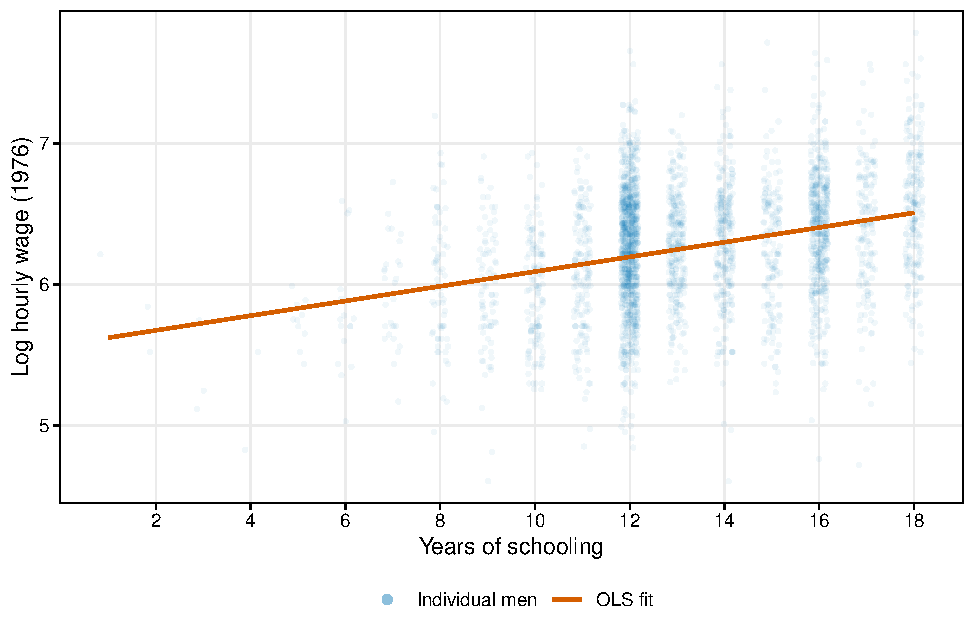
\includegraphics[width=\linewidth]{fig/fig1_education_wage_scatter.pdf}
  \figurenote{Each point is one of the 3,010 men. Years of schooling are
  jittered horizontally to reduce overplotting. The solid line is the linear
  fit from Model 1.}
  \label{fig:scatter}
\end{figure}

\begin{figure}[htbp]
  \caption{Estimated Return to One Year of Schooling Across Three Models}
  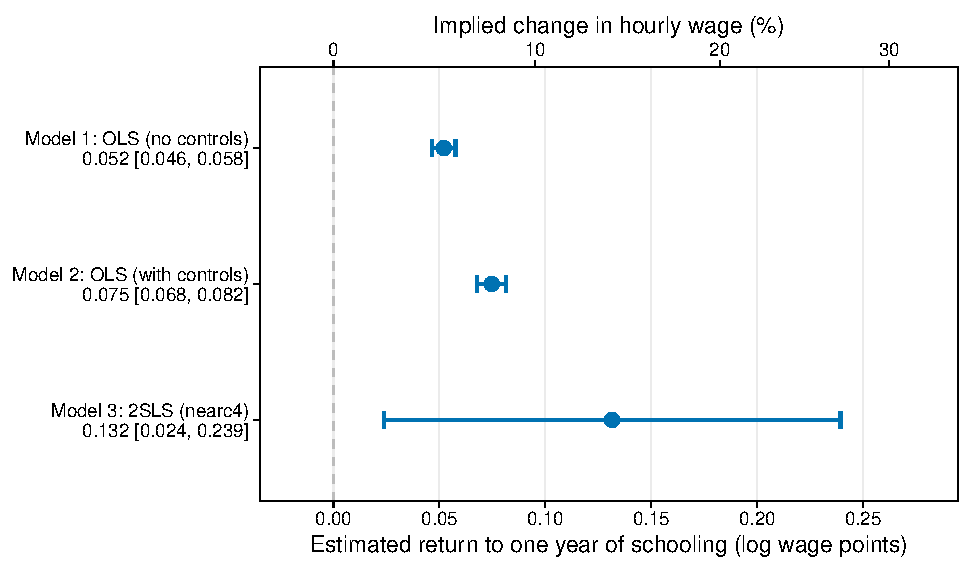
\includegraphics[width=\linewidth]{fig/fig2_returns_by_model.pdf}
  \figurenote{Points are point estimates and horizontal lines are 95\%
  confidence intervals. The dashed vertical line marks zero. Values below the
  model labels give the estimate and its 95\% confidence interval in log wage
  points. The top axis converts log wage points to the implied percentage
  change in hourly wages.}
  \label{fig:effects}
\end{figure}

\section{Discussion}

The replication recovers Card's central pattern. The OLS return is modest and
changes little when covariates are added, whereas the 2SLS estimate is
substantially larger. Under the exclusion restriction that college proximity
affects wages only through schooling, the gap is consistent with attenuation
from measurement error in self-reported schooling, and possibly with omitted
ability bias working in the opposite direction. The result therefore supports
Card's conclusion that conventional estimates may understate the economic value
of schooling.

The IV estimate is nevertheless fragile. The first-stage $F$ statistic is only
modestly above the conventional threshold of 10, and the 95\% confidence
interval for the 2SLS return is wide enough to include the OLS estimate. The
estimate is also a local average treatment effect: it applies to men whose
schooling decisions respond to college proximity, not to the population at
large. Finally, the exclusion restriction is not directly testable. College
proximity may proxy for local labor market conditions, school quality, or
family background, all of which could affect wages independently of schooling.

\section{Conclusion}

A single script reproduces the main estimates in \textcite{card1993} and
generates the figures, table, and results paragraph reported here. The exercise
shows both why college proximity is a useful source of identifying variation
and why cautious interpretation is warranted: the IV estimate is larger than
OLS, but it is imprecise and rests on a strong exclusion restriction.

\printbibliography

\end{document}
